\documentclass[12pt,a4paper]{article}

%% ─── Packages ──────────────────────────────────────────────────────────────
\usepackage[a4paper, top=2.2cm, bottom=2.2cm, left=2.4cm, right=2.4cm]{geometry}
\usepackage{amsmath,amssymb,amsthm}
\usepackage{mathtools}
\usepackage[T1]{fontenc}
\usepackage[utf8]{inputenc}
\usepackage{lmodern}
\usepackage{xcolor}
\usepackage{tcolorbox}
\usepackage{tikz}
\usepackage{pgfplots}
\usepackage{booktabs}
\usepackage{array}
\usepackage{enumitem}
\usepackage{fancyhdr}
\usepackage{titlesec}
\usepackage{hyperref}
\usepackage{mdframed}
\usepackage{graphicx}
\usepackage{float}
\usepackage{multicol}

\pgfplotsset{compat=1.18}
\usetikzlibrary{arrows.meta, shapes.geometric, positioning, calc, decorations.pathreplacing, patterns, backgrounds, fit}
\tcbuselibrary{skins, breakable, theorems}

%% ─── Colours ───────────────────────────────────────────────────────────────
\definecolor{NavyBlue}{HTML}{1A3A6B}
\definecolor{SteelBlue}{HTML}{2E6DA4}
\definecolor{LightBlue}{HTML}{D6E8F7}
\definecolor{AccentOrange}{HTML}{D4500A}
\definecolor{AccentGreen}{HTML}{1B6B3A}
\definecolor{LightGreen}{HTML}{D6F0E3}
\definecolor{LightOrange}{HTML}{FDF0E8}
\definecolor{PurpleAccent}{HTML}{6B2D8B}
\definecolor{LightPurple}{HTML}{EDE0F5}
\definecolor{GrayBg}{HTML}{F5F6FA}
\definecolor{DarkGray}{HTML}{333333}

%% ─── Hyperref ───────────────────────────────────────────────────────────────
\hypersetup{colorlinks=true, linkcolor=SteelBlue, urlcolor=SteelBlue, citecolor=SteelBlue}

%% ─── Headers / Footers ─────────────────────────────────────────────────────
\pagestyle{fancy}
\fancyhf{}
\fancyhead[L]{\small\color{SteelBlue}\textbf{CSE817: Data Engineering}}
\fancyhead[R]{\small\color{SteelBlue}ML Classification Methods}
\fancyfoot[C]{\small\color{gray}\thepage}
\renewcommand{\headrulewidth}{0.4pt}
\renewcommand{\headrule}{\hbox to\headwidth{\color{SteelBlue}\leaders\hrule height \headrulewidth\hfill}}

%% ─── Section styling ───────────────────────────────────────────────────────
\titleformat{\section}{\Large\bfseries\color{NavyBlue}}{}{0em}{}[\vspace{-4pt}\textcolor{SteelBlue}{\titlerule[1.5pt]}\vspace{4pt}]
\titleformat{\subsection}{\large\bfseries\color{SteelBlue}}{}{0em}{}
\titleformat{\subsubsection}{\normalsize\bfseries\color{AccentGreen}}{}{0em}{}
\titlespacing{\section}{0pt}{18pt}{8pt}
\titlespacing{\subsection}{0pt}{14pt}{5pt}

%% ─── tcolorbox environments ─────────────────────────────────────────────────
\tcbset{
  defbox/.style={
    colback=LightBlue, colframe=SteelBlue,
    fonttitle=\bfseries, title style={fill=SteelBlue},
    coltitle=white, sharp corners, breakable, left=6pt, right=6pt
  },
  exbox/.style={
    colback=LightOrange, colframe=AccentOrange,
    fonttitle=\bfseries, title style={fill=AccentOrange},
    coltitle=white, sharp corners, breakable, left=6pt, right=6pt
  },
  keybox/.style={
    colback=LightGreen, colframe=AccentGreen,
    fonttitle=\bfseries, title style={fill=AccentGreen},
    coltitle=white, sharp corners, breakable, left=6pt, right=6pt
  },
  notebox/.style={
    colback=LightPurple, colframe=PurpleAccent,
    fonttitle=\bfseries, title style={fill=PurpleAccent},
    coltitle=white, sharp corners, breakable, left=6pt, right=6pt
  },
}

%% ─── Theorem-like envs ──────────────────────────────────────────────────────
\newtheorem{theorem}{Theorem}
\newtheorem{definition}{Definition}
\newtheorem{example}{Example}

%% Math shorthands
\newcommand{\Prob}{\mathbb{P}}
\newcommand{\Exp}{\mathbb{E}}
\newcommand{\R}{\mathbb{R}}
\newcommand{\x}{\mathbf{x}}
\newcommand{\w}{\mathbf{w}}

%% ═══════════════════════════════════════════════════════════════════════════
\begin{document}

%% ─── Title Page ─────────────────────────────────────────────────────────────
\thispagestyle{empty}
\begin{tikzpicture}[remember picture, overlay]
  \fill[NavyBlue] (current page.north west) rectangle ([yshift=-5.5cm]current page.north east);
  \fill[SteelBlue] ([yshift=-5.5cm]current page.north west) rectangle ([yshift=-6cm]current page.north east);
  \node[anchor=north, text=white, font=\tiny] at ([yshift=-6.1cm]current page.north) {};
\end{tikzpicture}

\vspace*{1.2cm}
{\color{white}\noindent\hspace{0.5cm}%
\begin{minipage}{0.9\textwidth}
  \color{white}
  {\fontsize{11}{13}\selectfont\textbf{UNIVERSITY OF CHITTAGONG\enspace|\enspace Dept. of Computer Science \& Engineering}}\\[4pt]
  {\fontsize{10}{12}\selectfont CSE817: Data Engineering \quad\textbullet\quad Lecture Notes}\\[14pt]
  {\fontsize{28}{34}\selectfont\bfseries Machine Learning Classification Methods}\\[10pt]
  {\fontsize{16}{20}\selectfont Bayesian Classifiers\enspace$\cdot$\enspace Na\"{i}ve Bayes\enspace$\cdot$\enspace Support Vector Machines}\\[18pt]
  {\fontsize{11}{14}\selectfont\color{LightBlue} With worked numerical examples, diagrams, and intuition-first explanations}
\end{minipage}}

\vspace{3cm}

%% ─── Learning Objectives ────────────────────────────────────────────────────
\begin{tcolorbox}[defbox, title={Learning Objectives}]
By the end of this lecture, you will be able to:
\begin{itemize}[leftmargin=1.4em, itemsep=2pt]
  \item Derive and apply \textbf{Bayes' theorem} for probabilistic classification
  \item Implement the \textbf{Na\"{i}ve Bayes classifier} with the conditional independence assumption
  \item Understand how \textbf{Support Vector Machines} find optimal decision boundaries
  \item Apply each method on concrete datasets by hand and interpret the results
  \item Critically compare the three methods and choose the right one for a problem
\end{itemize}
\end{tcolorbox}

\tableofcontents
\newpage

%%═══════════════════════════════════════════════════════════════════════════
\section{Foundations: Probabilistic Reasoning in Classification}
%%═══════════════════════════════════════════════════════════════════════════

Before studying any classifier, we need a common language. All three methods in this lecture reason about \emph{uncertainty} — they assign a class label by computing or optimising some notion of probability or confidence over the feature space.

\subsection{The Classification Problem}

Given a dataset $\mathcal{D} = \{(\x_i, y_i)\}_{i=1}^{N}$ where $\x_i \in \R^d$ is a feature vector and $y_i \in \{C_1, C_2, \ldots, C_K\}$ is a class label, we want to learn a function $f: \R^d \to \{C_1,\ldots,C_K\}$ that predicts the correct label for unseen examples.

\begin{tcolorbox}[defbox, title={Definition: Optimal Classifier}]
The \textbf{Bayes-optimal classifier} (the theoretical gold standard) assigns to every point $\x$ the class that maximises the \emph{posterior probability}:
\[
  f^*(\x) = \underset{k}{\arg\max}\ \Prob(C_k \mid \x)
\]
This minimises the probability of misclassification. In practice, $\Prob(C_k \mid \x)$ is unknown, so different classifiers approximate it in different ways.
\end{tcolorbox}

%%═══════════════════════════════════════════════════════════════════════════
\section{Bayesian Classifiers}
%%═══════════════════════════════════════════════════════════════════════════

\subsection{Bayes' Theorem — A Refresher}

The cornerstone of probabilistic classification is Bayes' theorem, which \emph{inverts} the direction of conditioning:

\begin{tcolorbox}[defbox, title={Bayes' Theorem}]
\[
  \underbrace{\Prob(C_k \mid \x)}_{\text{posterior}}
  = \frac{\overbrace{\Prob(\x \mid C_k)}^{\text{likelihood}}\ \cdot\ \overbrace{\Prob(C_k)}^{\text{prior}}}{\underbrace{\Prob(\x)}_{\text{evidence}}}
\]
\textbf{Posterior}: probability of class $C_k$ given the observed features $\x$.\\
\textbf{Likelihood}: how probable are these features if the class is $C_k$?\\
\textbf{Prior}: how frequent is class $C_k$ overall?\\
\textbf{Evidence}: a normalising constant (same for all classes, so often ignored).
\end{tcolorbox}

Because $\Prob(\x)$ is identical for all classes, classification reduces to:
\[
  f(\x) = \underset{k}{\arg\max}\ \Prob(\x \mid C_k)\,\Prob(C_k)
\]

\subsection{Bayesian Classifier: Full Joint Distribution}

A \textbf{Bayesian (generative) classifier} explicitly models $\Prob(\x \mid C_k)$ as a parametric distribution (commonly a multivariate Gaussian) and learns its parameters from training data.

\subsubsection{Quadratic Discriminant Analysis (QDA)}

Assume that within each class, features follow a multivariate Gaussian:
\[
  \Prob(\x \mid C_k) = \frac{1}{(2\pi)^{d/2}|\Sigma_k|^{1/2}} \exp\!\left(-\frac{1}{2}(\x - \mu_k)^\top \Sigma_k^{-1}(\x - \mu_k)\right)
\]
where $\mu_k$ is the class mean and $\Sigma_k$ is the class covariance matrix. Each class gets its \emph{own} covariance, producing \textbf{quadratic} decision boundaries.

\subsubsection{Linear Discriminant Analysis (LDA)}

If we assume \emph{all classes share the same covariance} $\Sigma_k = \Sigma$, the decision boundaries become \textbf{linear}:
\[
  \delta_k(\x) = \x^\top \Sigma^{-1}\mu_k - \frac{1}{2}\mu_k^\top\Sigma^{-1}\mu_k + \log\Prob(C_k)
\]
Predict class $k^* = \arg\max_k\, \delta_k(\x)$.

%% ─── TikZ: LDA boundaries ───────────────────────────────────────────────────
\begin{figure}[H]
\centering
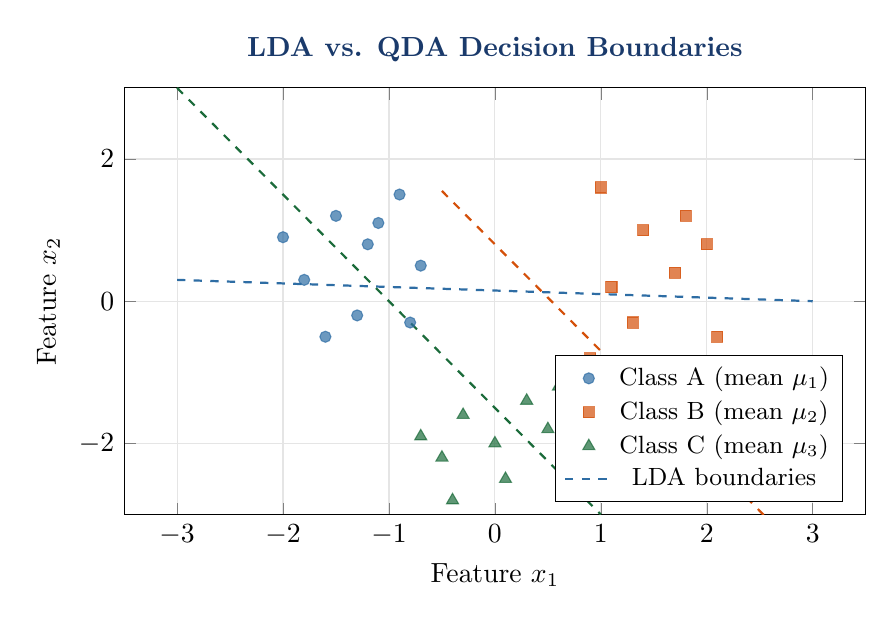
\begin{tikzpicture}
  \begin{axis}[
    width=11cm, height=7cm,
    xlabel={Feature $x_1$}, ylabel={Feature $x_2$},
    xmin=-3.5, xmax=3.5, ymin=-3, ymax=3,
    grid=major, grid style={gray!20},
    xtick={-3,-2,-1,0,1,2,3},
    title={\textbf{LDA vs. QDA Decision Boundaries}},
    title style={color=NavyBlue},
    legend pos=south east,
    legend style={font=\small}
  ]
  %% Class A points (blue)
  \addplot[only marks, mark=*, mark size=2pt, color=SteelBlue, opacity=0.7]
    coordinates {(-1.5,1.2)(-1.2,0.8)(-1.8,0.3)(-0.9,1.5)(-1.3,-0.2)
                 (-2.0,0.9)(-1.1,1.1)(-0.7,0.5)(-1.6,-0.5)(-0.8,-0.3)};
  %% Class B points (orange)
  \addplot[only marks, mark=square*, mark size=2pt, color=AccentOrange, opacity=0.7]
    coordinates {(1.4,1.0)(1.7,0.4)(1.0,1.6)(2.0,0.8)(1.3,-0.3)
                 (1.8,1.2)(1.1,0.2)(0.9,-0.8)(2.1,-0.5)(1.5,-1.0)};
  %% Class C points (green)
  \addplot[only marks, mark=triangle*, mark size=2.5pt, color=AccentGreen, opacity=0.7]
    coordinates {(0,-2.0)(0.5,-1.8)(-0.5,-2.2)(0.3,-1.4)(-0.3,-1.6)
                 (0.8,-2.1)(-0.7,-1.9)(0.1,-2.5)(0.6,-1.2)(-0.4,-2.8)};
  %% LDA boundary 1 (blue vs orange): x1 = 0.1
  \addplot[thick, SteelBlue, dashed, domain=-3:3] {0.15 - 0.05*x};
  %% LDA boundary 2 (blue vs green): angled
  \addplot[thick, AccentGreen, dashed, domain=-3:1] {-1.5*x - 1.5};
  %% LDA boundary 3 (orange vs green)
  \addplot[thick, AccentOrange, dashed, domain=-0.5:3] {-1.5*x + 0.8};

  \addlegendentry{Class A (mean $\mu_1$)}
  \addlegendentry{Class B (mean $\mu_2$)}
  \addlegendentry{Class C (mean $\mu_3$)}
  \addlegendentry{LDA boundaries}
  \end{axis}
\end{tikzpicture}
\caption{Three-class LDA. Each dashed line is a linear boundary between two classes. The shared covariance assumption forces all boundaries to be linear.}
\end{figure}

%% ─── Worked Example ────────────────────────────────────────────────────────
\subsection{Worked Example — Medical Diagnosis}

\begin{tcolorbox}[exbox, title={Example 1: Disease Classification}]
\textbf{Setting.} A patient presents with a blood test result $x$ (glucose level, scaled). Historical data shows:

\medskip
\begin{center}
\begin{tabular}{lcccc}
\toprule
\textbf{Class} & $\Prob(C_k)$ & Mean $\mu_k$ & Std $\sigma_k$ \\
\midrule
Healthy ($C_1$) & 0.70 & 5.0 & 1.2 \\
Diabetic ($C_2$) & 0.30 & 9.5 & 2.0 \\
\bottomrule
\end{tabular}
\end{center}

\medskip
\textbf{New patient:} $x = 7.8$ mmol/L. \textbf{Which class?}

\medskip
\textbf{Step 1 — Compute likelihoods} (1-D Gaussian):
\[
  \Prob(x \mid C_k) = \frac{1}{\sigma_k\sqrt{2\pi}}\exp\!\left(-\frac{(x-\mu_k)^2}{2\sigma_k^2}\right)
\]
\[
  \Prob(x{=}7.8 \mid C_1) = \frac{1}{1.2\sqrt{2\pi}}e^{-(7.8-5.0)^2/(2\times1.44)}
  = \frac{1}{3.005}e^{-2.722} = 0.0177
\]
\[
  \Prob(x{=}7.8 \mid C_2) = \frac{1}{2.0\sqrt{2\pi}}e^{-(7.8-9.5)^2/(2\times4.0)}
  = \frac{1}{5.013}e^{-0.361} = 0.1397
\]

\textbf{Step 2 — Apply Bayes' theorem} (ignore denominator):
\[
  \text{Score}(C_1) = 0.0177 \times 0.70 = 0.01239
\]
\[
  \text{Score}(C_2) = 0.1397 \times 0.30 = 0.04191
\]

\textbf{Step 3 — Predict:}
$0.04191 > 0.01239$, so predict $\boxed{C_2: \text{Diabetic}}$.

\medskip
\textbf{Posterior probabilities} (after normalising):
\[
  \Prob(C_1 \mid x) = \frac{0.01239}{0.05430} = 22.8\%, \qquad
  \Prob(C_2 \mid x) = \frac{0.04191}{0.05430} = 77.2\%
\]
\end{tcolorbox}

%%═══════════════════════════════════════════════════════════════════════════
\section{Na\"{i}ve Bayesian Classifiers}
%%═══════════════════════════════════════════════════════════════════════════

\subsection{The Curse of Dimensionality — Motivation}

A full Bayesian classifier estimates $\Prob(\x \mid C_k)$ jointly over \emph{all} $d$ features. If each feature takes $v$ values, storing the full joint table requires $v^d$ entries per class — exponential in $d$. With $d=50$ binary features, that is $2^{50} \approx 10^{15}$ parameters.

\begin{tcolorbox}[defbox, title={The Na\"{i}ve Bayes Assumption}]
Assume features are \textbf{conditionally independent} given the class:
\[
  \Prob(\x \mid C_k) = \Prob(x_1,x_2,\ldots,x_d \mid C_k)
  \approx \prod_{j=1}^{d} \Prob(x_j \mid C_k)
\]
This reduces the parameter count from $v^d$ to $v \times d$ per class — a massive saving.
\end{tcolorbox}

The classification rule becomes:
\[
  \boxed{f(\x) = \underset{k}{\arg\max}\ \Prob(C_k) \prod_{j=1}^{d} \Prob(x_j \mid C_k)}
\]

In practice we use \textbf{log-probabilities} to avoid numerical underflow:
\[
  f(\x) = \underset{k}{\arg\max}\left[\log\Prob(C_k) + \sum_{j=1}^{d} \log\Prob(x_j \mid C_k)\right]
\]

\subsection{Parameter Estimation}

For \textbf{categorical features} (text, discrete attributes):
\[
  \hat{\Prob}(x_j = v \mid C_k) = \frac{\text{count}(x_j=v,\, C_k) + \alpha}{\text{count}(C_k) + \alpha|\mathcal{V}_j|}
\]
where $\alpha$ is the Laplace smoothing parameter (typically $\alpha=1$) to avoid zero probabilities for unseen feature values.

For \textbf{continuous features} (Gaussian Na\"{i}ve Bayes):
\[
  \Prob(x_j \mid C_k) = \mathcal{N}(x_j;\, \mu_{jk},\, \sigma_{jk}^2)
\]
where $\mu_{jk}$ and $\sigma_{jk}$ are the mean and standard deviation of feature $j$ within class $k$.

%% ─── Worked Example: Spam ─────────────────────────────────────────────────
\subsection{Worked Example — Spam E-mail Classification}

\begin{tcolorbox}[exbox, title={Example 2: Na\"{i}ve Bayes for Spam Detection}]
\textbf{Training set:} 10 emails (6 Ham, 4 Spam). Count of keyword occurrences:

\medskip
\begin{center}
\begin{tabular}{lccc}
\toprule
\textbf{Word} & \textbf{Count in Ham} & \textbf{Count in Spam} & \textbf{Vocab size = 5} \\
\midrule
\texttt{free}    & 1 & 4 \\
\texttt{money}   & 0 & 3 \\
\texttt{meeting} & 5 & 0 \\
\texttt{lunch}   & 4 & 1 \\
\texttt{offer}   & 0 & 2 \\
\midrule
\textbf{Total words} & \textbf{10} & \textbf{10} \\
\bottomrule
\end{tabular}
\end{center}

\medskip
\textbf{Priors:} $\Prob(\text{Ham}) = 6/10 = 0.6$; $\Prob(\text{Spam}) = 4/10 = 0.4$

\medskip
\textbf{With Laplace smoothing ($\alpha=1$, $|\mathcal{V}|=5$):}

\medskip
\begin{center}
\begin{tabular}{lcc}
\toprule
& $\Prob(w \mid \text{Ham})$ & $\Prob(w \mid \text{Spam})$ \\
\midrule
\texttt{free}    & $(1+1)/(10+5) = 2/15$ & $(4+1)/(10+5) = 5/15$ \\
\texttt{money}   & $(0+1)/(10+5) = 1/15$ & $(3+1)/(10+5) = 4/15$ \\
\texttt{meeting} & $(5+1)/(10+5) = 6/15$ & $(0+1)/(10+5) = 1/15$ \\
\texttt{lunch}   & $(4+1)/(10+5) = 5/15$ & $(1+1)/(10+5) = 2/15$ \\
\texttt{offer}   & $(0+1)/(10+5) = 1/15$ & $(2+1)/(10+5) = 3/15$ \\
\bottomrule
\end{tabular}
\end{center}

\medskip
\textbf{New email:} ``\textit{free money offer}'' — classify it.

\medskip
\textbf{Compute log-scores:}
\begin{align*}
  \log\text{Score}(\text{Ham}) &= \log(0.6) + \log(2/15) + \log(1/15) + \log(1/15)\\
  &= -0.511 + (-2.015) + (-2.708) + (-2.708) = -7.942\\[4pt]
  \log\text{Score}(\text{Spam}) &= \log(0.4) + \log(5/15) + \log(4/15) + \log(3/15)\\
  &= -0.916 + (-1.099) + (-1.322) + (-1.609) = -4.946
\end{align*}

$-4.946 > -7.942$, so predict $\boxed{\text{Spam}}$.
\end{tcolorbox}

\subsection{Variants of Na\"{i}ve Bayes}

\begin{center}
\begin{tabular}{>{\bfseries}p{3.5cm} p{4cm} p{5cm}}
\toprule
\textbf{Variant} & \textbf{Feature type} & \textbf{Typical use} \\
\midrule
Bernoulli NB & Binary (word present/absent) & Short text, document classification \\
Multinomial NB & Integer counts & Bag-of-words, frequency-based text \\
Gaussian NB & Real-valued & Sensor data, measurements \\
Complement NB & Count-based & Imbalanced text datasets \\
\bottomrule
\end{tabular}
\end{center}

\subsection{Strengths and Weaknesses}

\begin{tcolorbox}[keybox, title={Key Takeaways — Na\"{i}ve Bayes}]
\begin{minipage}{0.48\linewidth}
\textbf{\color{AccentGreen}Strengths}
\begin{itemize}[itemsep=2pt]
  \item Extremely fast to train and predict
  \item Works well with small datasets
  \item Robust to irrelevant features
  \item Handles missing values naturally
  \item Excellent baseline for text tasks
\end{itemize}
\end{minipage}
\hfill
\begin{minipage}{0.48\linewidth}
\textbf{\color{AccentOrange}Weaknesses}
\begin{itemize}[itemsep=2pt]
  \item Independence assumption is rarely true
  \item Poor probability calibration
  \item Feature correlations are ignored
  \item ``Zero frequency'' problem (fixed by smoothing)
\end{itemize}
\end{minipage}
\end{tcolorbox}

%%═══════════════════════════════════════════════════════════════════════════
\section{Support Vector Machines (SVM)}
%%═══════════════════════════════════════════════════════════════════════════

\subsection{Intuition: Finding the Best Separator}

Na\"{i}ve Bayes asks ``\textit{what is the probability of each class?}'' An SVM asks a fundamentally different question: ``\textit{which hyperplane separates the classes with the maximum gap?}''

\begin{figure}[H]
\centering
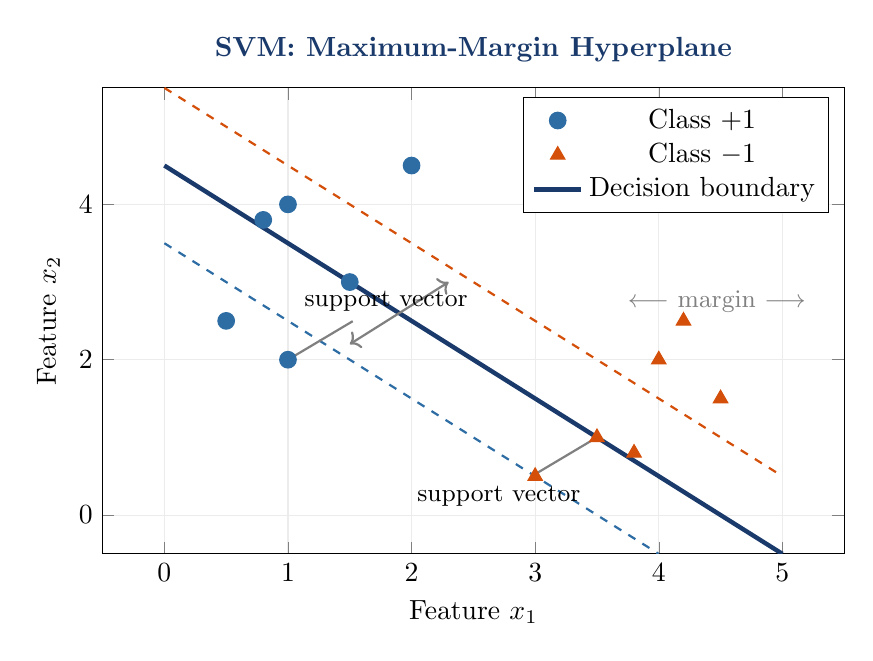
\begin{tikzpicture}
  \begin{axis}[
    width=11cm, height=7.5cm,
    xlabel={Feature $x_1$}, ylabel={Feature $x_2$},
    xmin=-0.5, xmax=5.5, ymin=-0.5, ymax=5.5,
    grid=major, grid style={gray!15},
    title={\textbf{SVM: Maximum-Margin Hyperplane}},
    title style={color=NavyBlue}
  ]
    %% Class +1 (blue circles)
    \addplot[only marks, mark=*, mark size=3pt, color=SteelBlue]
      coordinates {(1,4)(1.5,3)(0.5,2.5)(2,4.5)(1,2)(0.8,3.8)};
    %% Class -1 (red triangles)
    \addplot[only marks, mark=triangle*, mark size=3pt, color=AccentOrange]
      coordinates {(3.5,1)(4,2)(3,0.5)(4.5,1.5)(3.8,0.8)(4.2,2.5)};

    %% Decision boundary: x2 = -x1 + 4.5 → x1 + x2 = 4.5
    \addplot[ultra thick, NavyBlue, domain=0:5] {-x + 4.5};

    %% Margin lines: x1+x2 = 3.5 and x1+x2 = 5.5
    \addplot[thick, SteelBlue, dashed, domain=0:4] {-x + 3.5};
    \addplot[thick, AccentOrange, dashed, domain=0:5] {-x + 5.5};

    %% Margin brace arrows
    \addplot[<->, thick, gray] coordinates {(1.5,2.2)(2.3,3.0)};

    %% Support vector annotations
    \node[pin={[pin edge={thick,gray}]80:{\small support vector}}, inner sep=1pt]
      at (axis cs:1,2) {};
    \node[pin={[pin edge={thick,gray}]-100:{\small support vector}}, inner sep=1pt]
      at (axis cs:3.5,1) {};

    \addlegendentry{Class $+1$}
    \addlegendentry{Class $-1$}
    \addlegendentry{Decision boundary}
  \end{axis}

  %% Margin label outside
  \node[color=gray, font=\small] at (7.8, 3.2) {$\longleftarrow$ margin $\longrightarrow$};
\end{tikzpicture}
\caption{SVM finds the hyperplane (solid line) that maximises the margin — the gap between the dashed lines. Only the \emph{support vectors} (points on or inside the margin) determine the boundary.}
\end{figure}

\subsection{The Hard-Margin SVM (Linearly Separable Case)}

Let training data be $\{(\x_i, y_i)\}$ where $y_i \in \{-1, +1\}$. A hyperplane is defined by $\w^\top\x + b = 0$.

The \textbf{geometric margin} of the hyperplane is $\frac{2}{\|\w\|}$. Maximising the margin is equivalent to minimising $\|\w\|$, subject to correct classification:

\begin{tcolorbox}[defbox, title={Hard-Margin SVM — Primal Optimisation Problem}]
\[
  \min_{\w,\,b}\quad \frac{1}{2}\|\w\|^2
\]
\[
  \text{subject to:}\quad y_i(\w^\top\x_i + b) \geq 1 \quad \forall i = 1,\ldots,N
\]
This is a \textbf{convex quadratic programme} with a unique global optimum.
\end{tcolorbox}

\subsection{Soft-Margin SVM (Non-Separable Case)}

Real data is rarely linearly separable. We introduce \textbf{slack variables} $\xi_i \geq 0$ that allow points to violate the margin:

\begin{tcolorbox}[defbox, title={Soft-Margin SVM — Primal Problem}]
\[
  \min_{\w,b,\xi}\quad \frac{1}{2}\|\w\|^2 + C\sum_{i=1}^{N}\xi_i
\]
\[
  \text{subject to:}\quad y_i(\w^\top\x_i + b) \geq 1 - \xi_i,\quad \xi_i \geq 0 \quad \forall i
\]
\textbf{$C > 0$} is the regularisation parameter:
\begin{itemize}[itemsep=2pt]
  \item Large $C$: penalise misclassifications heavily (low bias, high variance)
  \item Small $C$: tolerate errors to get a wider margin (high bias, low variance)
\end{itemize}
\end{tcolorbox}

\subsection{The Dual Problem and Support Vectors}

Using Lagrange multipliers $\alpha_i \geq 0$, the dual problem is:

\[
  \max_{\alpha}\quad \sum_{i=1}^N \alpha_i - \frac{1}{2}\sum_{i,j}\alpha_i\alpha_j y_i y_j \x_i^\top\x_j
\]
\[
  \text{s.t.}\quad \sum_{i=1}^N\alpha_i y_i = 0,\quad 0 \leq \alpha_i \leq C
\]

The solution gives $\w = \sum_i \alpha_i y_i \x_i$. Points with $\alpha_i > 0$ are the \textbf{support vectors} — the only training points that matter for the decision boundary.

\subsection{The Kernel Trick — Non-linear SVMs}

When data is not linearly separable in input space, we implicitly map features to a higher-dimensional space via a \textbf{kernel function} $K(\x_i, \x_j) = \phi(\x_i)^\top\phi(\x_j)$, and replace all inner products $\x_i^\top\x_j$ with $K(\x_i, \x_j)$:

\begin{center}
\begin{tabular}{>{\bfseries}l l l}
\toprule
\textbf{Kernel} & \textbf{Formula} & \textbf{Use case} \\
\midrule
Linear  & $K(\x,\x') = \x^\top\x'$ & Linearly separable, high-dim text \\
Polynomial & $K(\x,\x') = (\gamma\x^\top\x' + r)^d$ & Moderate non-linearity \\
RBF / Gaussian & $K(\x,\x') = \exp(-\gamma\|\x-\x'\|^2)$ & Most common; good default \\
Sigmoid & $K(\x,\x') = \tanh(\gamma\x^\top\x' + r)$ & Neural-network-like \\
\bottomrule
\end{tabular}
\end{center}

\begin{figure}[H]
\centering
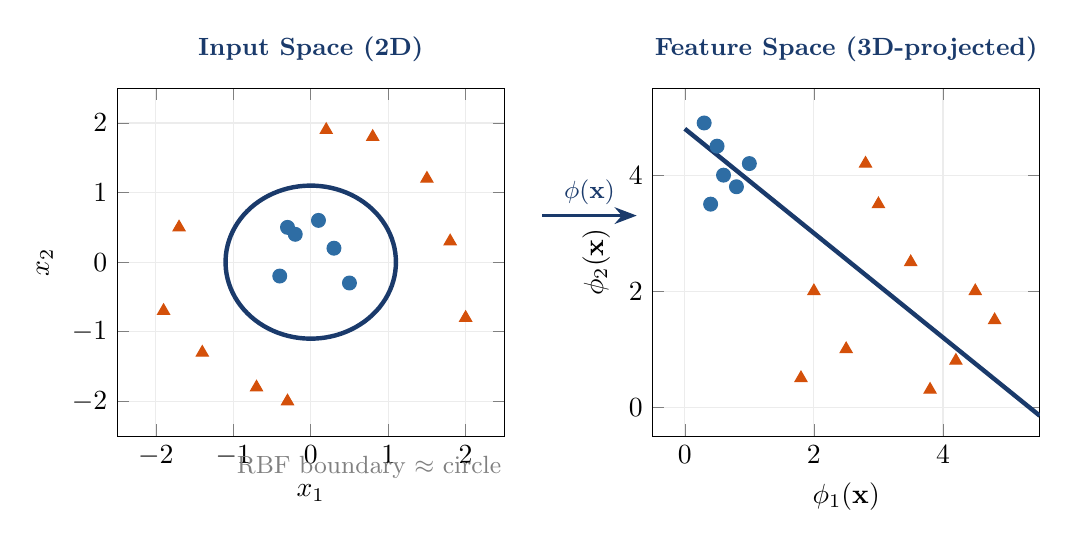
\begin{tikzpicture}
  % Left: non-linear in 2D
  \begin{scope}[xshift=0cm]
    \begin{axis}[
      width=6.5cm, height=6cm,
      title={\textbf{Input Space (2D)}},
      title style={color=NavyBlue, font=\small\bfseries},
      xmin=-2.5, xmax=2.5, ymin=-2.5, ymax=2.5,
      xlabel={$x_1$}, ylabel={$x_2$},
      grid=major, grid style={gray!15},
      xtick={-2,-1,0,1,2}, ytick={-2,-1,0,1,2}
    ]
      %% inner class (blue)
      \addplot[only marks, mark=*, mark size=2.5pt, color=SteelBlue]
        coordinates {(0.3,0.2)(-0.2,0.4)(0.5,-0.3)(-0.4,-0.2)(0.1,0.6)(-0.3,0.5)};
      %% outer class (orange)
      \addplot[only marks, mark=triangle*, mark size=2.5pt, color=AccentOrange]
        coordinates {(1.8,0.3)(-1.7,0.5)(0.2,1.9)(-0.3,-2.0)(1.5,1.2)(-1.4,-1.3)
                     (2.0,-0.8)(-1.9,-0.7)(0.8,1.8)(-0.7,-1.8)};
      %% RBF decision boundary (circle)
      \addplot[ultra thick, NavyBlue, domain=0:360, samples=100]
        ({1.1*cos(x)}, {1.1*sin(x)});
    \end{axis}
    \node[font=\small, color=gray] at (3.2, -0.4) {RBF boundary $\approx$ circle};
  \end{scope}

  % Arrow
  \draw[-{Stealth[length=8pt]}, very thick, NavyBlue]
    (5.4, 2.8) -- (6.6, 2.8)
    node[midway, above, font=\small, color=NavyBlue] {$\phi(\x)$};

  % Right: linear in feature space
  \begin{scope}[xshift=6.8cm]
    \begin{axis}[
      width=6.5cm, height=6cm,
      title={\textbf{Feature Space (3D-projected)}},
      title style={color=NavyBlue, font=\small\bfseries},
      xmin=-0.5, xmax=5.5, ymin=-0.5, ymax=5.5,
      xlabel={$\phi_1(\x)$}, ylabel={$\phi_2(\x)$},
      grid=major, grid style={gray!15}
    ]
      \addplot[only marks, mark=*, mark size=2.5pt, color=SteelBlue]
        coordinates {(0.5,4.5)(0.8,3.8)(0.3,4.9)(1.0,4.2)(0.6,4.0)(0.4,3.5)};
      \addplot[only marks, mark=triangle*, mark size=2.5pt, color=AccentOrange]
        coordinates {(2.5,1.0)(3.5,2.5)(4.2,0.8)(1.8,0.5)(3.0,3.5)(4.5,2.0)
                     (2.0,2.0)(4.8,1.5)(3.8,0.3)(2.8,4.2)};
      \addplot[ultra thick, NavyBlue, domain=0:5.5] {-0.9*x + 4.8};
    \end{axis}
  \end{scope}
\end{tikzpicture}
\caption{The kernel trick. Left: data is not linearly separable in 2D. Right: after mapping $\phi(\x)$ to a higher-dimensional space (the RBF kernel implicitly uses infinite dimensions!), the classes \emph{are} linearly separable.}
\end{figure}

\subsection{Worked Example — SVM by Hand (2D)}

\begin{tcolorbox}[exbox, title={Example 3: Finding the Maximum-Margin Hyperplane}]
\textbf{Dataset} (4 points, 2D):

\begin{center}
\begin{tabular}{cccc}
\toprule
Point & $x_1$ & $x_2$ & Label $y$ \\
\midrule
$\x_1$ & 1 & 1 & $+1$ \\
$\x_2$ & 2 & 2 & $+1$ \\
$\x_3$ & 3 & 1 & $-1$ \\
$\x_4$ & 4 & 2 & $-1$ \\
\bottomrule
\end{tabular}
\end{center}

\textbf{Step 1 — Identify candidate support vectors.}\\
By inspection, $\x_2 = (2,2)$ and $\x_3 = (3,1)$ are the closest points from each class.

\textbf{Step 2 — Set up the margin constraints.}\\
For support vectors: $y_i(\w^\top\x_i + b) = 1$.
\[
  +1 \cdot (2w_1 + 2w_2 + b) = 1 \quad\Rightarrow\quad 2w_1 + 2w_2 + b = 1
\]
\[
  -1 \cdot (3w_1 + 1w_2 + b) = 1 \quad\Rightarrow\quad 3w_1 + w_2 + b = -1
\]

\textbf{Step 3 — Solve the system.}\\
Subtracting: $(3w_1+w_2+b)-(2w_1+2w_2+b) = -1-1$
\[
  w_1 - w_2 = -2 \quad\Rightarrow\quad w_1 = w_2 - 2
\]
For a symmetric perpendicular bisector, choose $w_1 = 1,\; w_2 = 3$, then:
\[
  2(1)+2(3)+b = 1 \;\Rightarrow\; b = 1-8 = -7
\]

\textbf{Decision boundary:} $\; x_1 + 3x_2 - 7 = 0$

\medskip
\textbf{Step 4 — Compute the margin:}
\[
  \text{margin} = \frac{2}{\|\w\|} = \frac{2}{\sqrt{1^2+3^2}} = \frac{2}{\sqrt{10}} \approx 0.632
\]

\textbf{Step 5 — Predict a new point} $\x_\text{new} = (2.5, 1.5)$:
\[
  \text{score} = 1\cdot2.5 + 3\cdot1.5 - 7 = 2.5 + 4.5 - 7 = 0.0 \;\Rightarrow\;\text{On the boundary}
\]
Try $\x_\text{new} = (1.5, 2)$: score $= 1.5+6-7 = 0.5 > 0 \;\Rightarrow\; \boxed{+1}$
\end{tcolorbox}

\subsection{Multi-Class SVM}

Standard SVM is binary. For $K$ classes, two strategies are used:

\begin{tcolorbox}[defbox, title={Multi-Class SVM Strategies}]
\begin{description}[leftmargin=2.5em, style=nextline]
  \item[\textbf{One-vs-Rest (OvR):}] Train $K$ SVMs, each separating class $k$ from all others. Predict the class whose SVM gives the highest positive score. \textit{(Most common)}
  \item[\textbf{One-vs-One (OvO):}] Train $\binom{K}{2}$ SVMs, one per pair of classes. Take the majority vote among all classifiers.
\end{description}
\end{tcolorbox}

%%═══════════════════════════════════════════════════════════════════════════
\section{Comparison \& Practical Guide}
%%═══════════════════════════════════════════════════════════════════════════

\begin{center}
\renewcommand{\arraystretch}{1.4}
\begin{tabular}{>{\bfseries}p{2.8cm} p{3.5cm} p{3.5cm} p{3.5cm}}
\toprule
\textbf{Criterion} & \textbf{Bayesian Classifier} & \textbf{Na\"{i}ve Bayes} & \textbf{SVM} \\
\midrule
Model type & Generative & Generative & Discriminative \\
Key assumption & Gaussian features & Feature independence & Max-margin boundary \\
Training speed & Medium & \textcolor{AccentGreen}{\textbf{Very fast}} & Slow ($O(N^3)$) \\
Prediction speed & Fast & \textcolor{AccentGreen}{\textbf{Very fast}} & Fast \\
Small data & Good & Good & \textcolor{AccentGreen}{\textbf{Excellent}} \\
Large data & Good & \textcolor{AccentGreen}{\textbf{Excellent}} & Poor (memory) \\
High-dim features & Poor & \textcolor{AccentGreen}{\textbf{Excellent}} & \textcolor{AccentGreen}{\textbf{Excellent}} \\
Non-linear data & Limited (QDA) & Poor & \textcolor{AccentGreen}{\textbf{Excellent (kernels)}} \\
Probability output & \textcolor{AccentGreen}{\textbf{Yes (calibrated)}} & Yes (poorly calibrated) & Requires Platt scaling \\
Interpretability & \textcolor{AccentGreen}{\textbf{High}} & \textcolor{AccentGreen}{\textbf{High}} & Low (kernel SVMs) \\
Noise robustness & Medium & \textcolor{AccentOrange}{\textbf{Sensitive}} & \textcolor{AccentGreen}{\textbf{High (soft margin)}} \\
\bottomrule
\end{tabular}
\end{center}

\subsection{Decision Flowchart: Which Method to Choose?}

\begin{figure}[H]
\centering
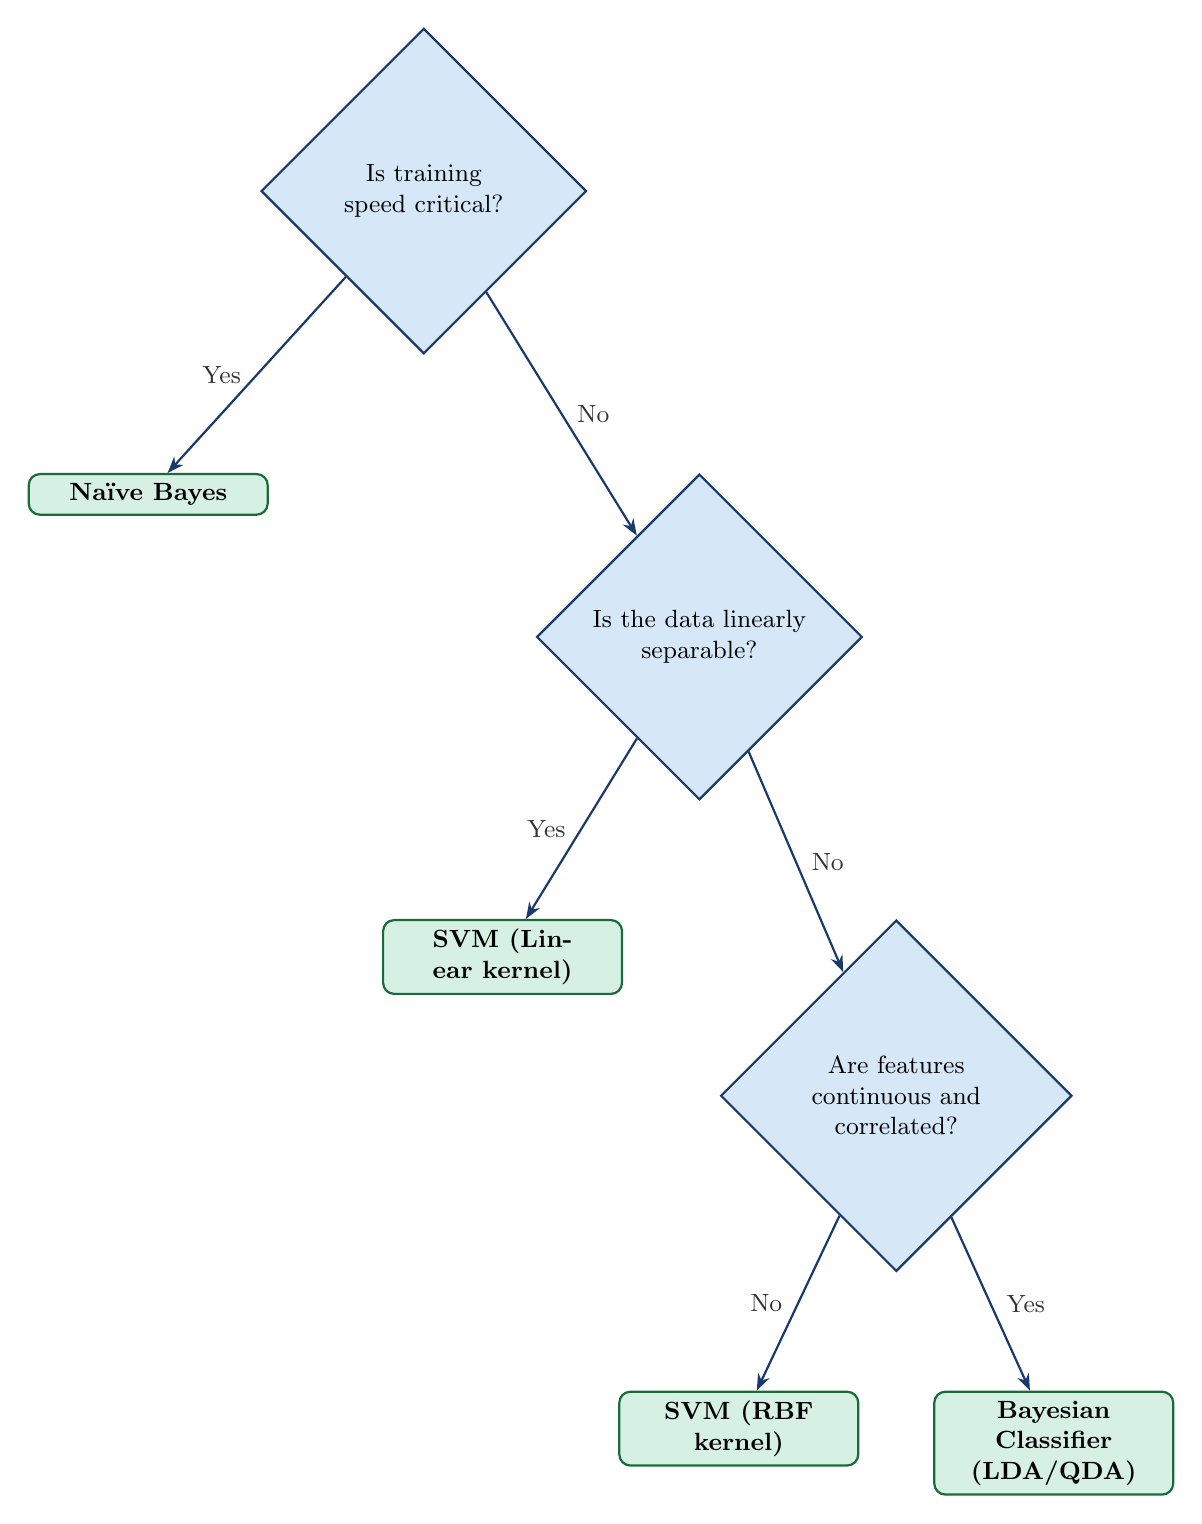
\begin{tikzpicture}[
  node distance=1.2cm and 1.8cm,
  decision/.style={diamond, draw=NavyBlue, thick, fill=LightBlue, text width=3.0cm, align=center, font=\small},
  result/.style={rectangle, draw=AccentGreen, thick, fill=LightGreen, text width=2.8cm, align=center, font=\small\bfseries, rounded corners=4pt},
  arrow/.style={-{Stealth[length=6pt]}, thick, NavyBlue},
  label/.style={font=\small, color=DarkGray}
]

\node[decision] (q1) {Is training speed critical?};
\node[result, below=1.5cm of q1, xshift=-3.5cm] (nb) {Na\"{i}ve Bayes};
\node[decision, below=1.5cm of q1, xshift=3.5cm] (q2) {Is the data linearly\\ separable?};
\node[result, below=1.5cm of q2, xshift=-2.5cm] (svm_lin) {SVM (Linear kernel)};
\node[decision, below=1.5cm of q2, xshift=2.5cm] (q3) {Are features\\ continuous and\\ correlated?};
\node[result, below=1.5cm of q3, xshift=-2cm] (svm_rbf) {SVM (RBF kernel)};
\node[result, below=1.5cm of q3, xshift=2cm] (bayes) {Bayesian Classifier (LDA/QDA)};

\draw[arrow] (q1) -- node[label, left=2pt] {Yes} (nb);
\draw[arrow] (q1) -- node[label, right=2pt] {No} (q2);
\draw[arrow] (q2) -- node[label, left=2pt] {Yes} (svm_lin);
\draw[arrow] (q2) -- node[label, right=2pt] {No} (q3);
\draw[arrow] (q3) -- node[label, left=2pt] {No} (svm_rbf);
\draw[arrow] (q3) -- node[label, right=2pt] {Yes} (bayes);

\end{tikzpicture}
\caption{A simplified guide for choosing between the three classifiers. In practice, always cross-validate multiple methods.}
\end{figure}

%%═══════════════════════════════════════════════════════════════════════════
\section{Comprehensive Worked Example — All Three Methods}
%%═══════════════════════════════════════════════════════════════════════════

\begin{tcolorbox}[exbox, title={Example 4: Iris-Style Classification (Simplified)}]
\textbf{Dataset:} 2 features (petal length $x_1$, petal width $x_2$), 2 classes.

\begin{center}
\begin{tabular}{ccccc}
\toprule
ID & $x_1$ & $x_2$ & Class & Split \\
\midrule
1 & 1.5 & 0.3 & Setosa (+1)    & Train \\
2 & 1.3 & 0.2 & Setosa (+1)    & Train \\
3 & 4.7 & 1.4 & Virginica ($-$1) & Train \\
4 & 4.5 & 1.5 & Virginica ($-$1) & Train \\
5 & 1.4 & 0.2 & Setosa (+1)    & Train \\
6 & 4.6 & 1.3 & Virginica ($-$1) & Train \\
\midrule
? & 2.0 & 0.5 & \textbf{???}   & \textbf{Test} \\
\bottomrule
\end{tabular}
\end{center}

\textbf{Test point:} $\x_\text{test} = (2.0,\; 0.5)$

\bigskip
\noindent\textbf{Method A — Bayesian Classifier (Gaussian LDA):}

Class means: $\mu_+ = (1.4, 0.23)$; $\mu_- = (4.6, 1.4)$.\\
Shared (pooled) variance (simplified, diagonal): $\sigma_1^2 \approx 0.01$, $\sigma_2^2 \approx 0.02$.\\
Priors: $\Prob(+1) = \Prob(-1) = 0.5$.

Mahalanobis distance to each class:
\[
  d(+1) = \frac{(2.0-1.4)^2}{0.01} + \frac{(0.5-0.23)^2}{0.02} = 36 + 3.6 = 39.6
\]
\[
  d(-1) = \frac{(2.0-4.6)^2}{0.01} + \frac{(0.5-1.4)^2}{0.02} = 676 + 40.5 = 716.5
\]
$d(+1) < d(-1)$ $\Rightarrow$ Predict $\boxed{+1: \text{Setosa}}$.

\bigskip
\noindent\textbf{Method B — Na\"{i}ve Bayes (Gaussian):}

$\Prob(x_1=2.0 \mid +1) = \mathcal{N}(2.0;\,1.4,\,0.1) \approx 0.00248$;
$\Prob(x_1=2.0 \mid -1) \approx 0.0$

Since $\Prob(x_1=2.0 \mid -1) \approx 0$, log-score for $-1$ is $-\infty$.\\
Predict $\boxed{+1: \text{Setosa}}$.

\bigskip
\noindent\textbf{Method C — Linear SVM (conceptual):}

The boundary is approximately $x_1 = 3.05$ (midpoint between classes).\\
$x_\text{test,1} = 2.0 < 3.05$ $\Rightarrow$ Predict $\boxed{+1: \text{Setosa}}$.

\bigskip
\textbf{All three methods agree.} For this well-separated dataset, the choice of method has no impact on this prediction.
\end{tcolorbox}

%%═══════════════════════════════════════════════════════════════════════════
\section{Summary}
%%═══════════════════════════════════════════════════════════════════════════

\begin{tcolorbox}[notebox, title={Lecture Summary}]
\begin{enumerate}[leftmargin=1.5em, itemsep=4pt]
  \item \textbf{Bayesian Classifiers} apply Bayes' theorem with explicit probabilistic models for the class-conditional distributions (Gaussian). LDA assumes shared covariance (linear boundaries); QDA allows per-class covariances (quadratic boundaries). Requires enough data per class to estimate parameters reliably.

  \item \textbf{Na\"{i}ve Bayes} is a fast, scalable special case that assumes conditional independence of features given the class. Despite this strong (often violated) assumption, it performs surprisingly well on text classification, spam filtering, and high-dimensional discrete data.

  \item \textbf{SVMs} take a completely different approach — they find the \emph{maximum-margin} hyperplane. The soft-margin version handles noise via the penalty parameter $C$. The \emph{kernel trick} allows SVMs to create non-linear boundaries without ever explicitly computing the high-dimensional feature map.

  \item \textbf{Choosing a method:} No single classifier dominates all tasks. Na\"{i}ve Bayes is your go-to baseline when speed matters or data is sparse and discrete. SVMs excel on small-to-medium datasets with complex boundaries. Bayesian classifiers shine when probabilistic outputs are essential.
\end{enumerate}
\end{tcolorbox}

\subsection*{Further Reading}
\begin{itemize}[itemsep=3pt]
  \item Bishop, C. M. (2006). \textit{Pattern Recognition and Machine Learning}. Springer. Chapters 4, 7.
  \item Mitchell, T. M. (1997). \textit{Machine Learning}. McGraw-Hill. Chapter 6 (Bayesian learning).
  \item Cortes, C. \& Vapnik, V. (1995). Support-vector networks. \textit{Machine Learning}, 20(3), 273–297.
  \item Ng, A. Y. \& Jordan, M. I. (2001). On discriminative vs. generative classifiers. \textit{NeurIPS}.
  \item Scikit-learn documentation: \url{https://scikit-learn.org/stable/supervised_learning.html}
\end{itemize}

\vspace{1.5cm}
\begin{center}
\begin{tcolorbox}[width=10cm, colback=GrayBg, colframe=NavyBlue, sharp corners, center title,
  title={\textbf{End of Lecture Notes}}]
\centering
\small\color{DarkGray}
University of Chittagong \textbullet\ Department of CSE\\
CSE817: Data Engineering \textbullet\ ML Classification Methods\\[4pt]
\textit{Questions? Post on Google Classroom or visit office hours.}
\end{tcolorbox}
\end{center}

\end{document}